Para consultar todos los objetos de un subárbol de la MIB utilizamos el comando \textbf{snmpwalk}.\\

Se muestran los dos primeros campos que corresponden a los dos OIDs del índice de cada uno de los dos nucleos de procesador que le fueron asignados a la máquina virtual en la que está corriendo el sistema operativo Ubuntu 18.04. Los otros dos datos corresponden a los objetos hrProcessorFrwID y hrProcessorLoad.

\pagebreak
\begin{figure}[!htpb]
	\hypertarget{fig:tarea3}{\hspace{1pt}}
	\begin{center}
		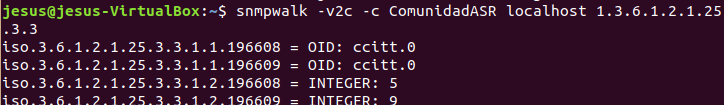
\includegraphics{imagenes/tarea3.png}
		\caption{Se muestran los objetos de la MIB correspondientdes a la tabla hrProcessorTable.}
		\label{fig:tarea3}	
	\end{center}
\end{figure}